\documentclass[11pt]{article}
\usepackage[margin=1in]{geometry}  % set the margins to 1in on all sides
\usepackage{graphicx}              % to include figures
\usepackage{amsmath}               % great math stuff
\usepackage{amsfonts}              % for blackboard bold, etc
\usepackage{amsthm}                % better theorem environments
\usepackage{makeidx}               % index
\usepackage[utf8]{inputenc}        % now we have tildes!
\usepackage{graphicx}
\usepackage{wrapfig}
\usepackage[english]{babel}
\usepackage{color}
\usepackage{listings}
\usepackage{indentfirst}
\usepackage{multirow}

\graphicspath{{diagrams/}}

% Set more space after the equation display to make text more readable
\expandafter\def\expandafter\normalsize\expandafter{%
    \normalsize
    \setlength\abovedisplayskip{100pt}
    \setlength\belowdisplayskip{20pt}
    \setlength\abovedisplayshortskip{3pt}
    \setlength\belowdisplayshortskip{20pt}
}

\definecolor{dkgreen}{rgb}{0,0.6,0}
\definecolor{gray}{rgb}{0.5,0.5,0.5}
\definecolor{mauve}{rgb}{0.58,0,0.82}

\lstset{frame=tb,
  language=Python,
  aboveskip=3mm,
  belowskip=3mm,
  showstringspaces=false,
  columns=flexible,
  basicstyle={\small\ttfamily},
  numbers=left,
  numberstyle=\tiny\color{gray},
  keywordstyle=\color{blue},
  commentstyle=\color{dkgreen},
  stringstyle=\color{mauve},
  breaklines=true,
  breakatwhitespace=true,
  tabsize=3
}

\begin{document}

\begin{center}
  \Huge\textbf{Using Self-Organizing Maps to solve Travelling Salesman
    Problem}\\
  \vspace{1cm}
  \large\textsc{Maximilian Leonard Kleinhans \& Diego Vicente Martín}
\end{center}

\section{System Overview}

The goal of this system is to use Self-Organizing Maps to solve the Travelling
Salesman Problem. To achieve that, we will create a population of neurons that
is spatially distributed on a ring structure and as the algorithm progresses,
neurons are pulled towards the cities. By defining a 1D neighborhood in this 2D
space, we will make sure that the population behaves as an elastic ring that
stretches until it occupies all the cities, while it tries to keep the perimeter
as short as possible. Once we achieve it, we only have to traverse the cities
following the ring to obtain a TSP solution.\\

The main component of the system is located in \texttt{som.py}: First we scale
down the data, so that for each city coordinate $ c= (x, y) ~ 0 \le x,y \le 1$
holds true. Further is here the main execution loop located. In each iteration,
we pick a random city. Then we compute the best matching unit, that is closest
neuron to this city. That neuron, and its neighborhood, will be updated
following the formula:

$$
w_v(s+1) \; \leftarrow \;
w_v(s) + \alpha (s) \cdot \eta (u, v, s) \cdot (D(t) - w_v)
$$

Where $s$ is the iteration in which the neuron $w_u$ has been chosen as the
winner of the city $D(t)$, and the formula is used to update all the neurons
$w_v$ located in its neighborhood. The parameters in the formula are the
learning rate $\alpha(s)$,  the neighborhood function  $\eta(u, v, s)$. We also
have to remark that those last parameters decay over time. These weights
associated to each vector are initialized in our system to random values that
will be easily corrected through the first iterations, there is no point in
wasting time or computations in finding different ways to initialize the
network.\\

To achieve decaying, we will use different types of decay functions, that are
represented in the \texttt{decay.py} file: static decay (that maintains the same
value for that parameter through all the iterations), linear decay (that linearly
decreases the value of the parameter), or exponential decay (that exponentially
decays the value of the parameter). For convenience, these parameters have been
implemented as classes that can be passed to the computation methods.\\

The calculation of a TSP solution from a list of neuron is done as described in
chapter 4 in the compendium. That is, for each city we select the closest neuron
and then define the city order through the order of the selected neurons.\\

Also relevant to the system is to notice that we have implemented two different
neighborhood functions: \texttt{bubble}, constant in the while neighborhood, 0
elsewhere and \text{gaussian}, that creates a Gaussian distribution around the
winner. Both implementations can be found in the file
\texttt{neighborhood.py}.\\

Apart from these computation files, we also have implemented helper methods for
reading data sets from files and managing user input  in \texttt{helper.py}.
Furthermore also methods for plotting and saving snapshots of the system at
different moments of the execution, to see how the system gets to a certain
solution.\\


\section{Tuning the System}

Once the system was implemented, we still had to work with it to get good
results. Different combinations of parameters lay different results,
and we had to be comprehensive when testing for parameters.\\

As a general conclusion, static decay is generally not a good decay approach to
use. By keeping the parameters with a static value during all the execution is
much harder to make the system converge into a solution. It is still possible to
get decent results, but overall it is not worth to use static decay. If, in the
other hand, we use linear, we can see the system converging much better to a
certain solution: in the beginning the system tries different strategies to then
focus on fixing the small details of the chosen one. More or less the same
approach can be seen with exponential, but thanks to its nature it is able to
stabilize much faster than linear. That's why, overall, the best decay strategy
to use is exponential although linear can also lay great results (specially when
applied to the learning rate alone). Another conclusion we can make is, that
with increasing number of cities linear performs worse and in case of the
\texttt{uruguay} data set with 734 cities we could not get decent results using
linear decay.\\

Regarding neighborhood functions, the one that lays the best result is the
Gaussian function. Although bubble does not lay bad results, we can see how
Gaussian moves the network in a much softer fashion, due to its gradient to the
edges versus the 1 or 0 values or bubble. Nevertheless bubble is much faster to
compute and for increasing number of cities it might be more suitable in terms
of runtime.\\

Other parameters to be tuned are the initial value of learning rates and
neighbourhood size, although that depends on great part on the data set and the
decay function we are going to use: static will need lower values and we will be
able to use higher values at the beginning if we use a decay strategy. We also
have to think about the size of the population of neurons. As a general rule, we
will need more neurons than cities so we can model the path through all the
cities in the map. As we have been able to test, the optimal size of the
population to get a network with a proper size is about 4-8 times greater than
the city population of the data set.\\

\newpage

By doing this tuning, we got to the conclusion that this was the best parameters
for each of the decay strategies:

\begin{table}[ht]
  \begin{center}
    \begin{tabular}{| c | c | c | c | c | c | c | c |}
      \hline
      Map & Decay & Neurons/City & $N$
      & $\eta$ & $\alpha$ & Radius & Final Distance\\
      \hline
      \hline
      \multirow{3}{*}{\textbf{Western Sahara}}
        & Static & 6 & 5000 & Gaussian & 0.3 & 5 & 34814.67 \\
        & Linear & 8 & 500 & Gaussian & 0.7 & 23 & 27620.78 \\
        & Exponential & 8 & 500 & Gaussian & 0.7 & 23 & 27601.17 \\
      \hline
      \multirow{3}{*}{\textbf{Djibouti}}
        & Static & 4 & 5000 & Gaussian & 0.2 & 10 & 7692.15\\
        & Linear & 8 & 5000 & Gaussian & 0.7 & 71 & 6659.91 \\
        & Exponential & 8 & 1000 & Gaussian & 0.7 & 71 & 6659.91 \\
      \hline
      \multirow{3}{*}{\textbf{Qatar}}
        & Static & 6 & 5000 & Gaussian & 0.4 & 50 & 14678.38 \\
        & Linear & 8 & 10000 & Gaussian & 0.7 & 155 &10284.41 \\
        & Exponential & 8 & 5000 & Gaussian & 0.9 & 155 & 10195.32 \\
      \hline
      \multirow{3}{*}{\textbf{Uruguay}}
        & Static & 8 & 10000 & Gaussian & 0.4 & 500 & 357201.05 \\
        & Linear & 8 & 10000 & Gaussian & 0.9 & 587 & 141536.50 \\
        & Exponential & 8 & 10000 & Bubble & 0.7 & 587 & 86819.03 \\
      \hline
    \end{tabular}
  \end{center}
\end{table}

And these are the results of the paths found by the different executions:

\begin{figure}[!ht]
  \centering
  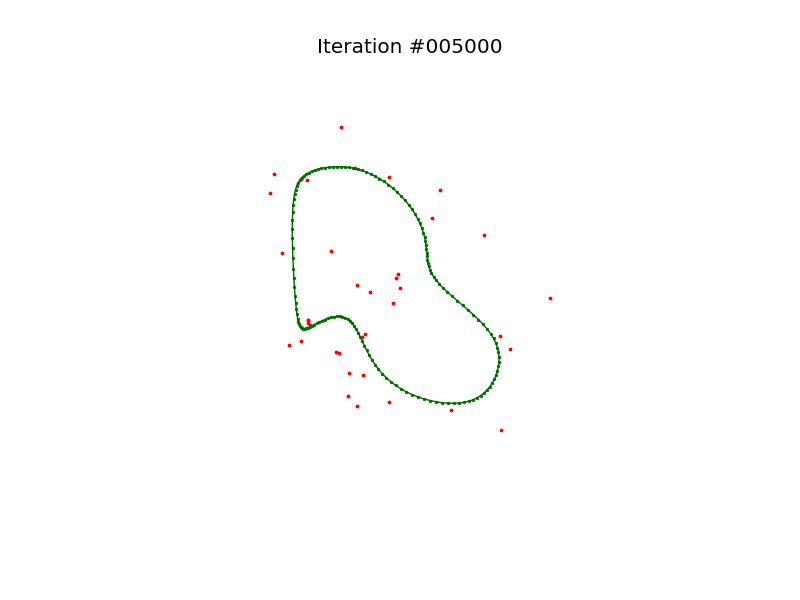
\includegraphics[scale=0.6]{d_s.png}
  \caption{Djibouti in Static Decay}
\end{figure}

\begin{figure}[!ht]
  \centering
  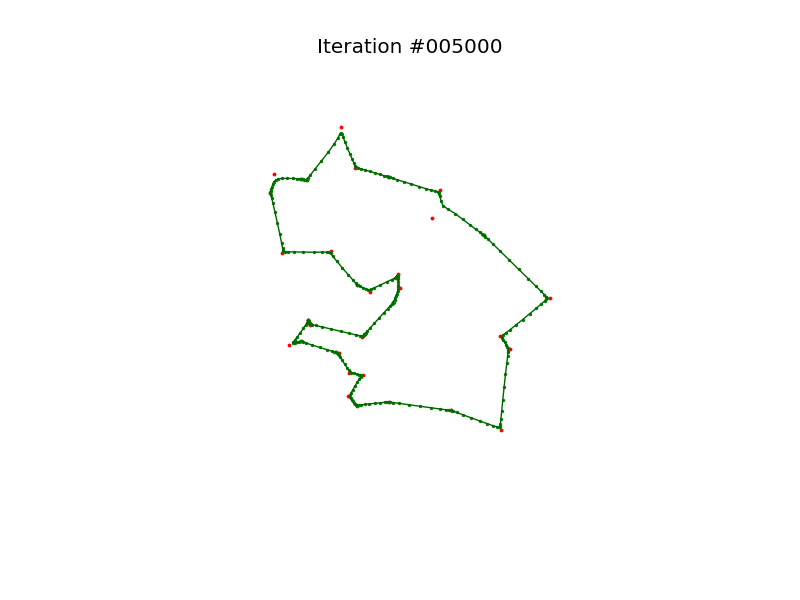
\includegraphics[scale=0.6]{d_l.png}
  \caption{Djibouti in Linear Decay}
\end{figure}

\begin{figure}[!ht]
  \centering
  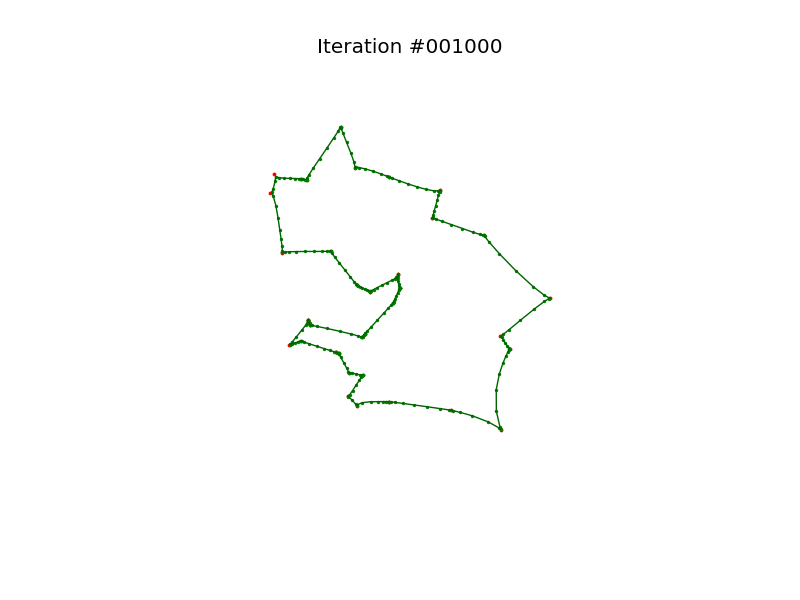
\includegraphics[scale=0.6]{d_e.png}
  \caption{Djibouti in Exponential Decay}
\end{figure}


\begin{figure}[!ht]
  \centering
  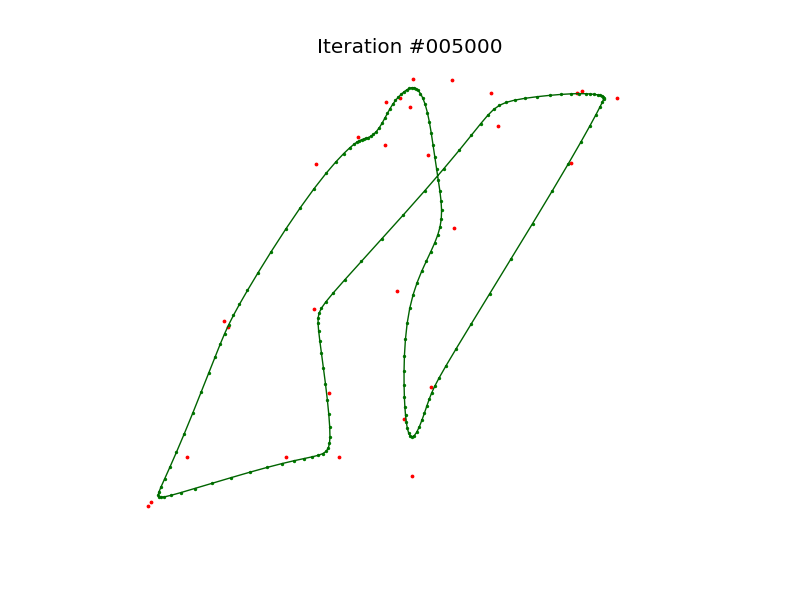
\includegraphics[scale=0.6]{w_s.png}
  \caption{Western Sahara in Static Decay}
\end{figure}

\begin{figure}[!ht]
  \centering
  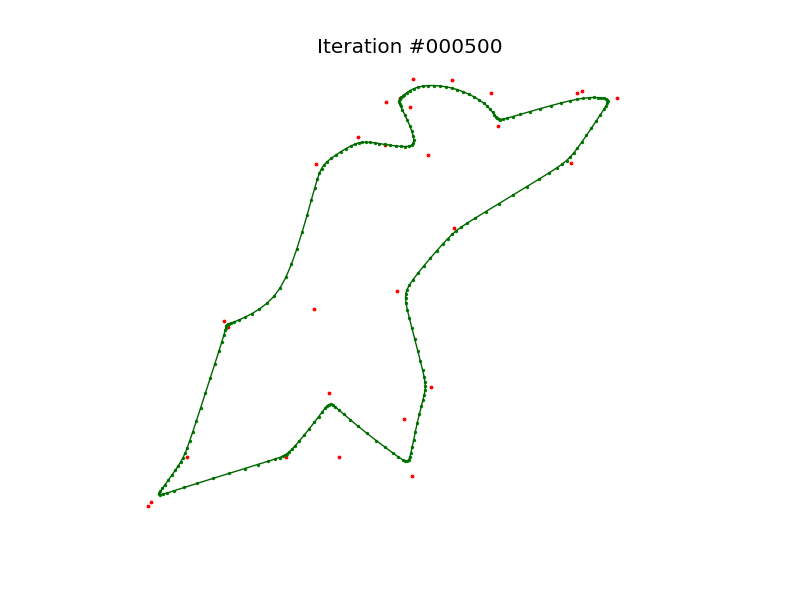
\includegraphics[scale=0.6]{w_l.png}
  \caption{Western Sahara in Linear Decay}
\end{figure}

\begin{figure}[!ht]
  \centering
  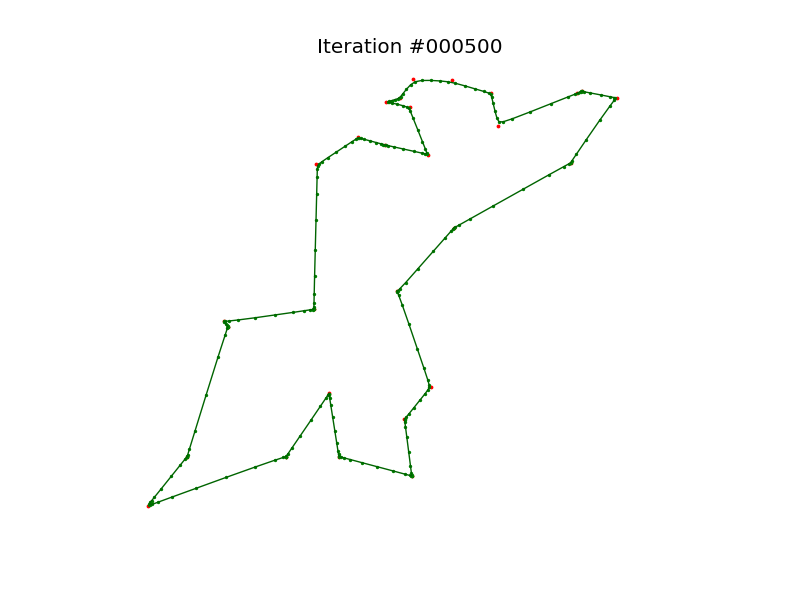
\includegraphics[scale=0.6]{w_e.png}
  \caption{Western Sahara in Exponential Decay}
\end{figure}


\begin{figure}[!ht]
  \centering
  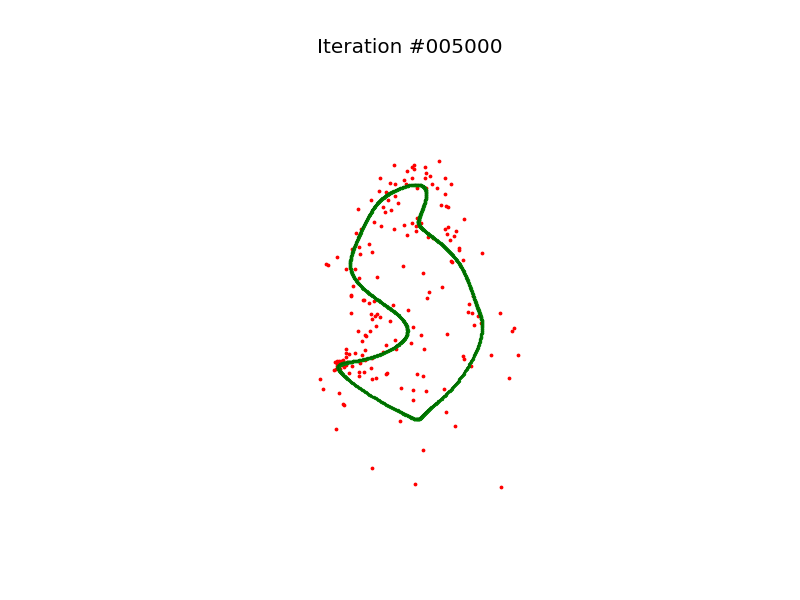
\includegraphics[scale=0.6]{q_s.png}
  \caption{Qatar in Static Decay}
\end{figure}

\begin{figure}[!ht]
  \centering
  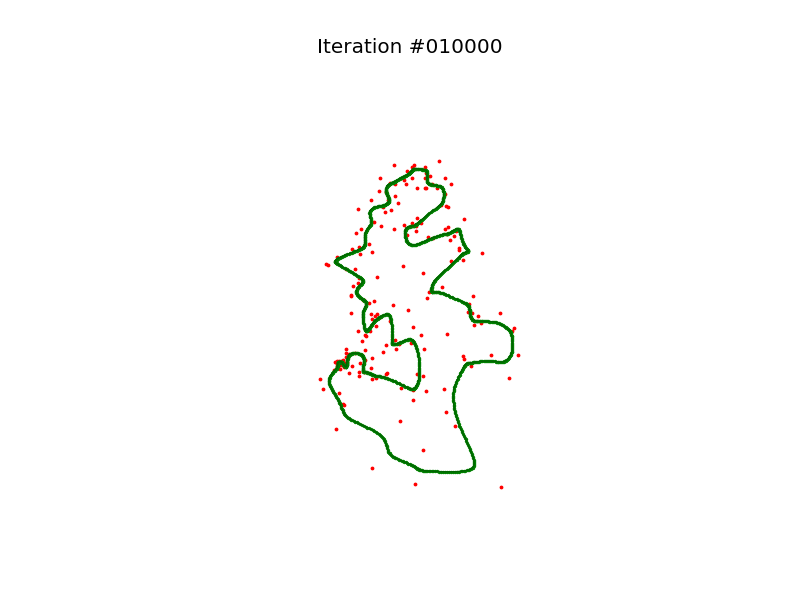
\includegraphics[scale=0.6]{q_l.png}
  \caption{Qatar in Linear Decay}
\end{figure}

\begin{figure}[!ht]
  \centering
  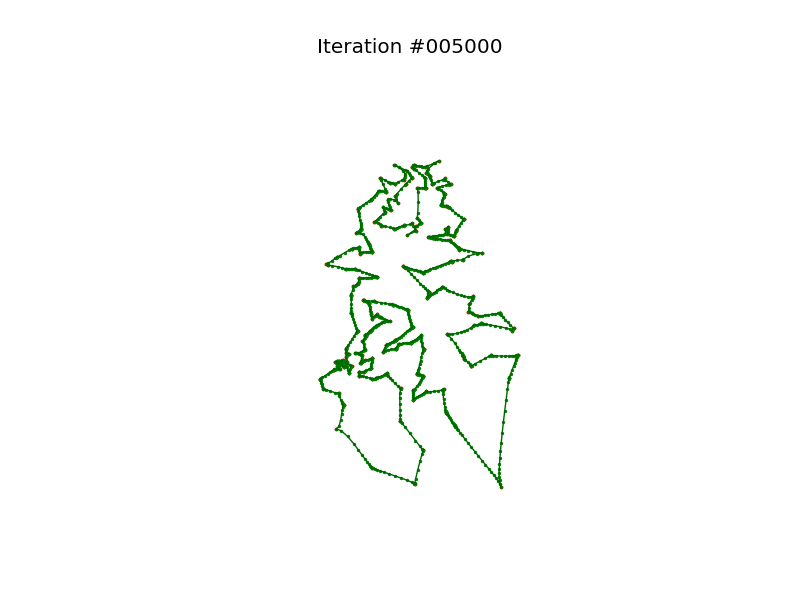
\includegraphics[scale=0.6]{q_e.png}
  \caption{Qatar in Exponential Decay}
\end{figure}


\begin{figure}[!ht]
  \centering
  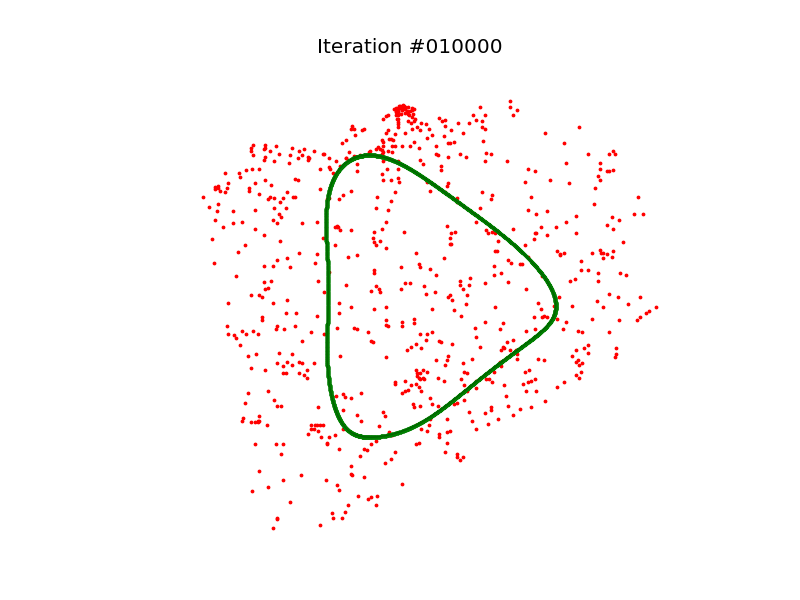
\includegraphics[scale=0.6]{u_s.png}
  \caption{Uruguay in Static Decay}
\end{figure}

\begin{figure}[!ht]
  \centering
  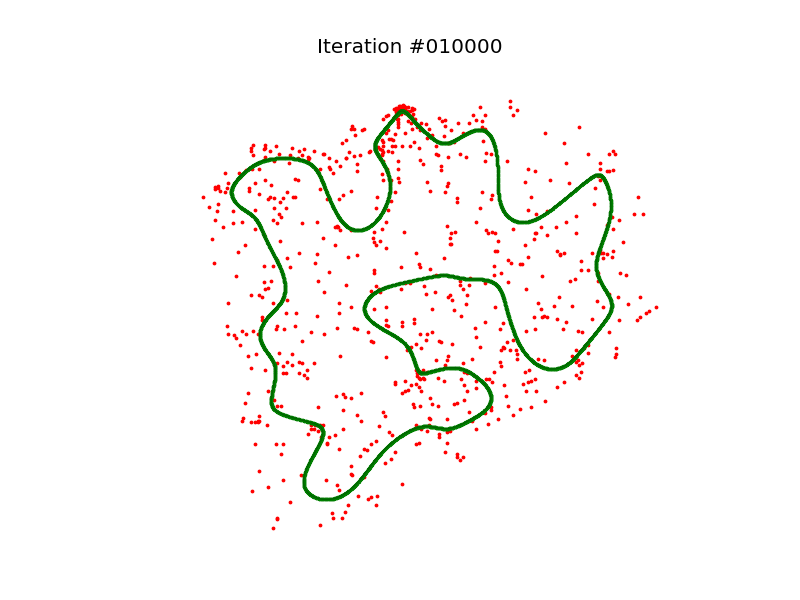
\includegraphics[scale=0.6]{u_l.png}
  \caption{Uruguay in Linear Decay}
\end{figure}

\begin{figure}[!ht]
  \centering
  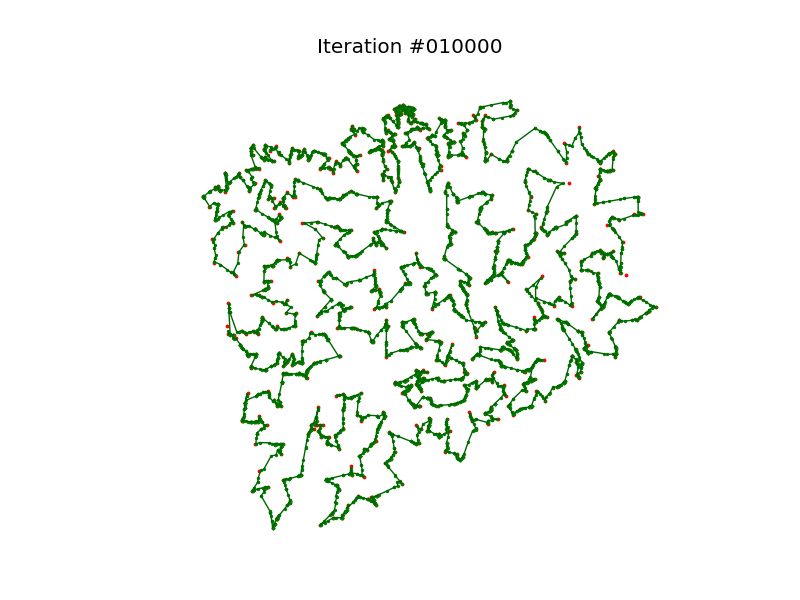
\includegraphics[scale=0.6]{u_e.png}
  \caption{Uruguay in Exponential Decay}
\end{figure}


\end{document}